% stack-perm-inout.tex

\documentclass{standalone}

\usepackage{tikz}
\usetikzlibrary{shapes, arrows.meta, positioning}

\begin{document}
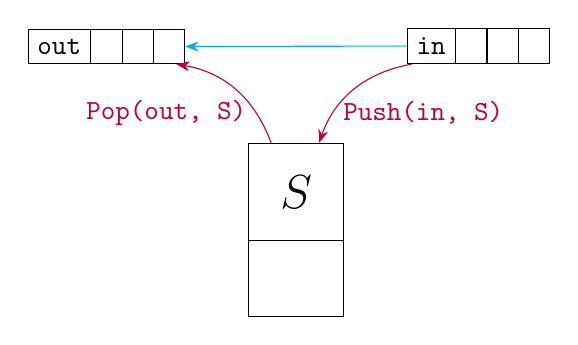
\begin{tikzpicture}[seq/.style = {rectangle split, 
  rectangle split horizontal, 
  rectangle split draw splits = true, 
  rectangle split parts = 4,
  draw}]

  \node[draw, rectangle split,
  	rectangle split parts = 2,
	inner sep = 4mm
      ] (stack) {\LARGE $S$};

  \node[seq, above right = 1.0cm and 0.8cm of stack] (in) {\texttt{in}};
  \node[seq, above left = 1.0cm and 0.8cm of stack] (out) {\texttt{out}};

  \draw[->, >=Stealth, bend right, purple] (in) to node[right, near end] {\texttt{Push(in, S)}} (stack);
  \draw[->, >=Stealth, bend right, purple] (stack) to node[left, near start] {\texttt{Pop(out, S)}} (out);

  \draw[->, >=Stealth, cyan] (in) to (out);
\end{tikzpicture}
\end{document}